% Standalone source for the method overview in pipeline.svg.
% Build with: latexmk -pdf assets/pipeline.tex
\documentclass[tikz,border=5pt]{standalone}
\usepackage{amsmath}
\usetikzlibrary{arrows.meta,positioning}

\begin{document}
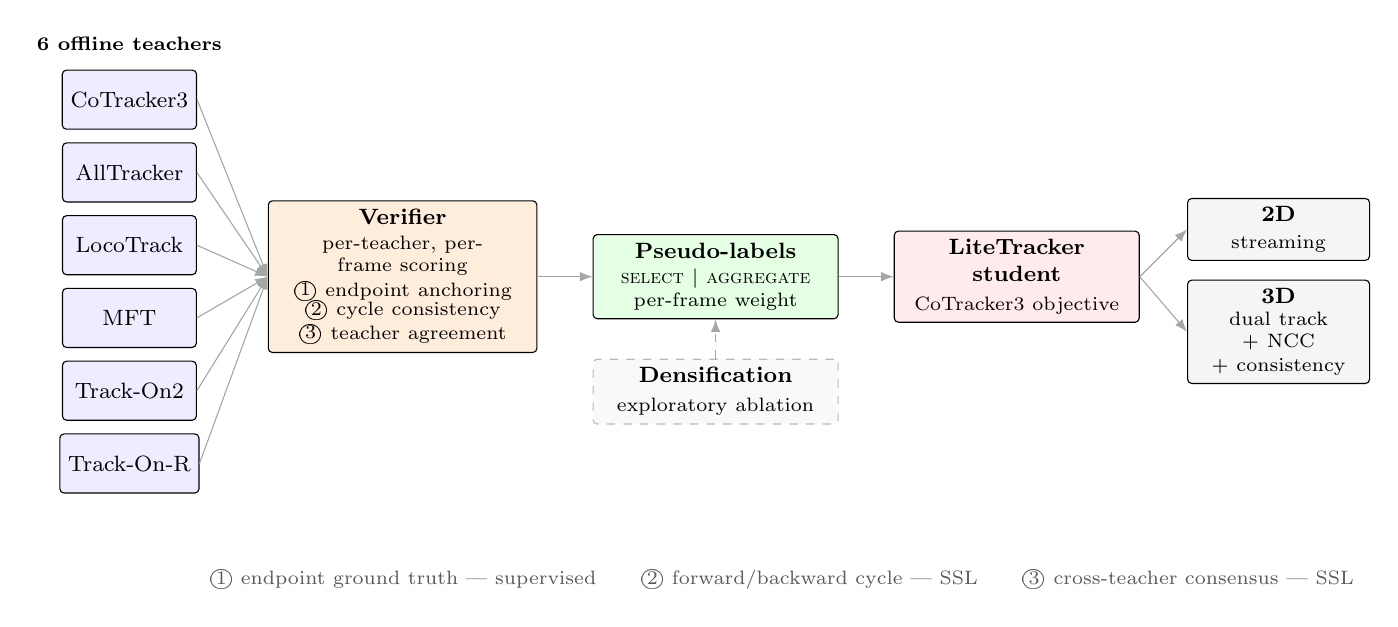
\begin{tikzpicture}[
  font=\footnotesize,
  node distance=3.2mm,
  box/.style={draw,rounded corners=1.5pt,align=center,inner sep=3pt,minimum height=7.5mm},
  t/.style={box,fill=blue!7,minimum width=17mm},
  v/.style={box,fill=orange!14,minimum width=32mm},
  d/.style={box,fill=green!10,minimum width=29mm},
  s/.style={box,fill=red!8,minimum width=29mm},
  ar/.style={-{Latex[length=1.6mm]},gray!70},
  experimental/.style={box,dashed,fill=gray!5,draw=gray!55,minimum width=29mm}]

\node[t] (t1) {CoTracker3};
\node[t,below=1.6mm of t1] (t2) {AllTracker};
\node[t,below=1.6mm of t2] (t3) {LocoTrack};
\node[t,below=1.6mm of t3] (t4) {MFT};
\node[t,below=1.6mm of t4] (t5) {Track-On2};
\node[t,below=1.6mm of t5] (t6) {Track-On-R};
\node[above=1.2mm of t1,font=\scriptsize\bfseries] {6 offline teachers};

\node[v,right=9mm of t3.east,yshift=-4mm,text width=32mm] (ver)
  {\textbf{Verifier}\\[1pt]
   \scriptsize per-teacher, per-frame scoring\\[1pt]
   \scriptsize \textcircled{1} endpoint anchoring\\[-1pt]
   \scriptsize \textcircled{2} cycle consistency\\[-1pt]
   \scriptsize \textcircled{3} teacher agreement};

\node[d,right=7mm of ver,text width=29mm] (pl)
  {\textbf{Pseudo-labels}\\[1pt]
   \scriptsize \textsc{select} $\mid$ \textsc{aggregate}\\[-1pt]
   \scriptsize per-frame weight};

\node[experimental,below=5mm of pl,text width=29mm] (dens)
  {\textbf{Densification}\\[1pt]
   \scriptsize exploratory ablation};

\node[s,right=7mm of pl,text width=29mm] (stu)
  {\textbf{LiteTracker student}\\[1pt]
   \scriptsize CoTracker3 objective};

\node[box,fill=gray!8,right=6mm of stu,text width=21mm,yshift=6mm] (mono)
  {\textbf{2D}\\\scriptsize streaming};
\node[box,fill=gray!8,right=6mm of stu,text width=21mm,yshift=-7mm] (ster)
  {\textbf{3D}\\\scriptsize dual track + NCC\\[-1pt]\scriptsize + consistency};

\foreach \n in {t1,t2,t3,t4,t5,t6} \draw[ar] (\n.east) -- (ver.west);
\draw[ar] (ver) -- (pl);
\draw[ar,dashed] (dens) -- (pl);
\draw[ar] (pl) -- (stu);
\draw[ar] (stu.east) -- (mono.west);
\draw[ar] (stu.east) -- (ster.west);

\node[below=11mm of t6.south east,anchor=west,font=\scriptsize,text=gray!70!black]
  {\textcircled{1} endpoint ground truth --- supervised\qquad
   \textcircled{2} forward/backward cycle --- SSL\qquad
   \textcircled{3} cross-teacher consensus --- SSL};
\end{tikzpicture}
\end{document}
